\documentclass[letterpaper,10pt,titlepage,draftclsnofoot,onecolumn,onesided] {IEEEtran}
\usepackage{listings}
\usepackage{underscore}
\usepackage[bookmarks=true]{hyperref}
\usepackage[utf8]{inputenc}
\usepackage[english]{babel}
\usepackage{hyperref}
\usepackage{titling}
\usepackage{graphicx}
\usepackage[noadjust]{cite}
\nocite{*}
\usepackage{abstract}
\graphicspath{ {images/} }

% Needed to get rid of "References" section in the TOC:
\makeatletter
\renewenvironment{thebibliography}[1]
     {\subsection*{\bibname}% <-- this line was changed from \chapter* to \section*
      \@mkboth{\MakeUppercase\bibname}{\MakeUppercase\bibname}%
      \list{\@biblabel{\@arabic\c@enumiv}}%
           {\settowidth\labelwidth{\@biblabel{#1}}%
            \leftmargin\labelwidth
            \advance\leftmargin\labelsep
            \@openbib@code
            \usecounter{enumiv}%
            \let\p@enumiv\@empty
            \renewcommand\theenumiv{\@arabic\c@enumiv}}%
      \sloppy
      \clubpenalty4000
      \@clubpenalty \clubpenalty
      \widowpenalty4000%
      \sfcode`\.\@m}
     {\def\@noitemerr
       {\@latex@warning{Empty `thebibliography' environment}}%
      \endlist}
\makeatother

\hypersetup{
    bookmarks=false,    % show bookmarks bar?
    pdftitle={Software Requirement Specification},    % title
    pdfauthor={Cramer Smith, Sam Lichlyter, Eric Winkler, Zach Schneider},                     % author
    pdfsubject={Requirements Document},                        % subject of the document
    pdfkeywords={IFT, Requirements, Postal}, % list of keywords
    colorlinks=true,       % false: boxed links; true: colored links
    linkcolor=black,       % color of internal links
    citecolor=black,       % color of links to bibliography
    filecolor=black,        % color of file links
    urlcolor=blue,        % color of external links
    linktoc=page            % only page is linked
} 

% Document Title:
\def\doctitle{A Tool to Automatically Organize the Structure of a Codebase Using Information Foraging Theory Design Patterns}
\def\doctype{Requirements Specifications Document}
\def\team{Team Postal}

\markboth{Oregon State University}{\doctitle}

\begin{document}

\title{\Huge{\bfseries{\textsf{\doctitle}}}\\\textsf{\Large{\doctype}}\\\textsf{\large{\team}}}
\author{Cramer Smith, Sam Lichlyter, Eric Winkler, Zach Schneider}

\maketitle
\vfill
%\begin{abstract}

\setlength\parindent{0pt} \textbf{Abstract:} Developer tools are often complex pieces of software. 
Gathering and manipulating useful information for a programmer can often be a slow and costly process. 
By implementing Information Foraging Theory design patterns in the creation of these tools, the information collected may be more useful or produced faster. 
Information Foraging Theory is the theory and math behind the choices people make to maximize the value of the information they find versus the cost of getting that information.
The aim of this project is to develop a tool that will act as a proof of concept to this idea and increase developer efficiency.
Through the implementation of multiple IFT design patterns, the Postal team will create a developer tool that helps enforce and maintain code structure. 

%\end{abstract}
\vfill

\pagebreak

\tableofcontents

\pagebreak

\section{Introduction}

The Postal extension is being made with two goals in mind.
The first is to provide evidence that the use of IFT Design Patterns in the production of developer tools is beneficial. 
The second is to create a tool that will help developers write and maintain clean code bases for websites.
The Postal extension will do this by giving the user reminders and suggestions about the best coding practices of the current language that they are using and by providing a visual representation of their project's code base.

\subsection{Purpose}
The purpose of the Software Requirements Specification of the Postal extension is to describe the extension's functionality and usage for the target user. 
This document will also help Team Postal and its stakeholders have a better understanding of the project's purpose and goals.

\subsection{Scope}
The Postal extension will be developed by Research Experience Undergraduates lead by Dr. Christopher Scaffidi. 
The project will be an extension for Visual Studio Code.
The purpose of this extension is to help new programmers develop good practices in their styling of code.
The extension will be aimed at new developers so that it will help them avoid  mistakes made during web development.
This extension will be able to parse the code that the user is editing and will be able to give them suggestions based on the current W3C standards. 

\subsection{Definitions, Acronyms, and Abbreviations}
\setlength\parindent{0pt} \textbf{Information Foraging Theory (IFT):} 
An approach to the analysis of human activities involving information access technologies.
The theory derives from optimal foraging theory in biology and anthropology, which analyzes the adaptive value of food-foraging strategies.\cite{xeroxift}\\\\
\textbf{IFT Design Patterns:} 
General, reusable solutions to common design problems.\cite{iftwiki}\\\\
\textbf{Visualize Topology:} 
To reveal the structure of the information topology to help developers more easily navigate structural relationships, backtrack, and make better decisions about which patches to visit.\cite{iftwiki}\\\\
\textbf{Notifier:} 
Automatically notify the developer of a change in an information patch which may result in prey desired by the developer appearing in the patch.\cite{iftwiki}\\\\
\textbf{Dashboard:} 
Generate an information patch in which a developer can become aware of links that lead to continually changing information patches relevant to his or her work.\cite{iftwiki}\\\\
\textbf{Gather Together:} 
Enable a developer to assemble information features from disparate patches into a single patch, thus reducing the cost of navigation between those features.\cite{iftwiki}\\\\
\textbf{Reduce Duplicate Information:} 
Enable developers to quickly forage by reducing the size of the topology. Here, the size of the topology is reduced by eliminating nodes with duplicate information.\cite{iftwiki}\\\\
\textbf{VSC, VS Code:}
Visual Studio Code.\\\\
\textbf{IRB:} 
Institutional Review Board.\\\\
\textbf{File Map:} 
The graphical user interface for visualizing project files and links, as well as errors inside code.\\\\
\textbf{Error List:}
A list which displays all errors that the parser detected during its last run.\\\\
\textbf{World Wide Web Consortium (W3C):}
The World Wide Web Consortium is an international community where Member organizations, a full-time staff, and the public work together to develop Web standards. \cite{w3}


%\subsection{References}

\begingroup
\bibliographystyle{IEEEtran}
\bibliography{requirements}
\endgroup

\subsection{Overview}
The remainder of this document will be concerned with the detailed requirements of Project Postal.
It will also describe what the Postal extension is specifically and how it will be used by developers.

\section{Overall Description}
Postal is an extension for Visual Studio code that will help entry-level developers while they make websites using HTML, CSS and JavaScript. 
The extension will parse the code they write and will assist in identifying errors or bad coding practice.

\subsection{Product Perspective}
The product is aimed toward individuals that are learning web development. This product aims for users to find that the tool makes the development process more educational and easier to understand. 
This checking tool differ from similar code checkers in that it will be offered in a free, cross-platform, light weight text editor.
This will make the correction and error identification more accessible to the users.

\subsubsection{System Interfaces}
Visual Studio Code was chosen as the sole system interface for Postal.
VSC is free, lightweight, cross-platform and open source, making it accessible to both developers and users of this development tool.

\subsubsection{User Interfaces}
The main interface that Team Postal plans to implement is a graphical representation of the user's files. 
Users will be able to quickly navigate through a visual representation of their files in the objective that this will give new developers a different way of thinking about their projects.
This different perspective will ideally encourage the user to implement better file structure and organization in their projects.

\subsubsection{Software Interfaces}
Development of this project requires interfacing with the VSC extension API. Development will utilize the Node Package Manager tool that is included in Node.js for initialization of the extension interface. The project will also use a code generator called yeoman to generate skeleton files which will edited and made into an extension using JavaScript. The skeleton code will be the base of what the rest of the extension is built on.

\subsubsection{Communication Interfaces}
The only communication interface that Postal will require is an ability to download the extension from the VS Code Extension Marketplace.

\begin{figure}
\centering
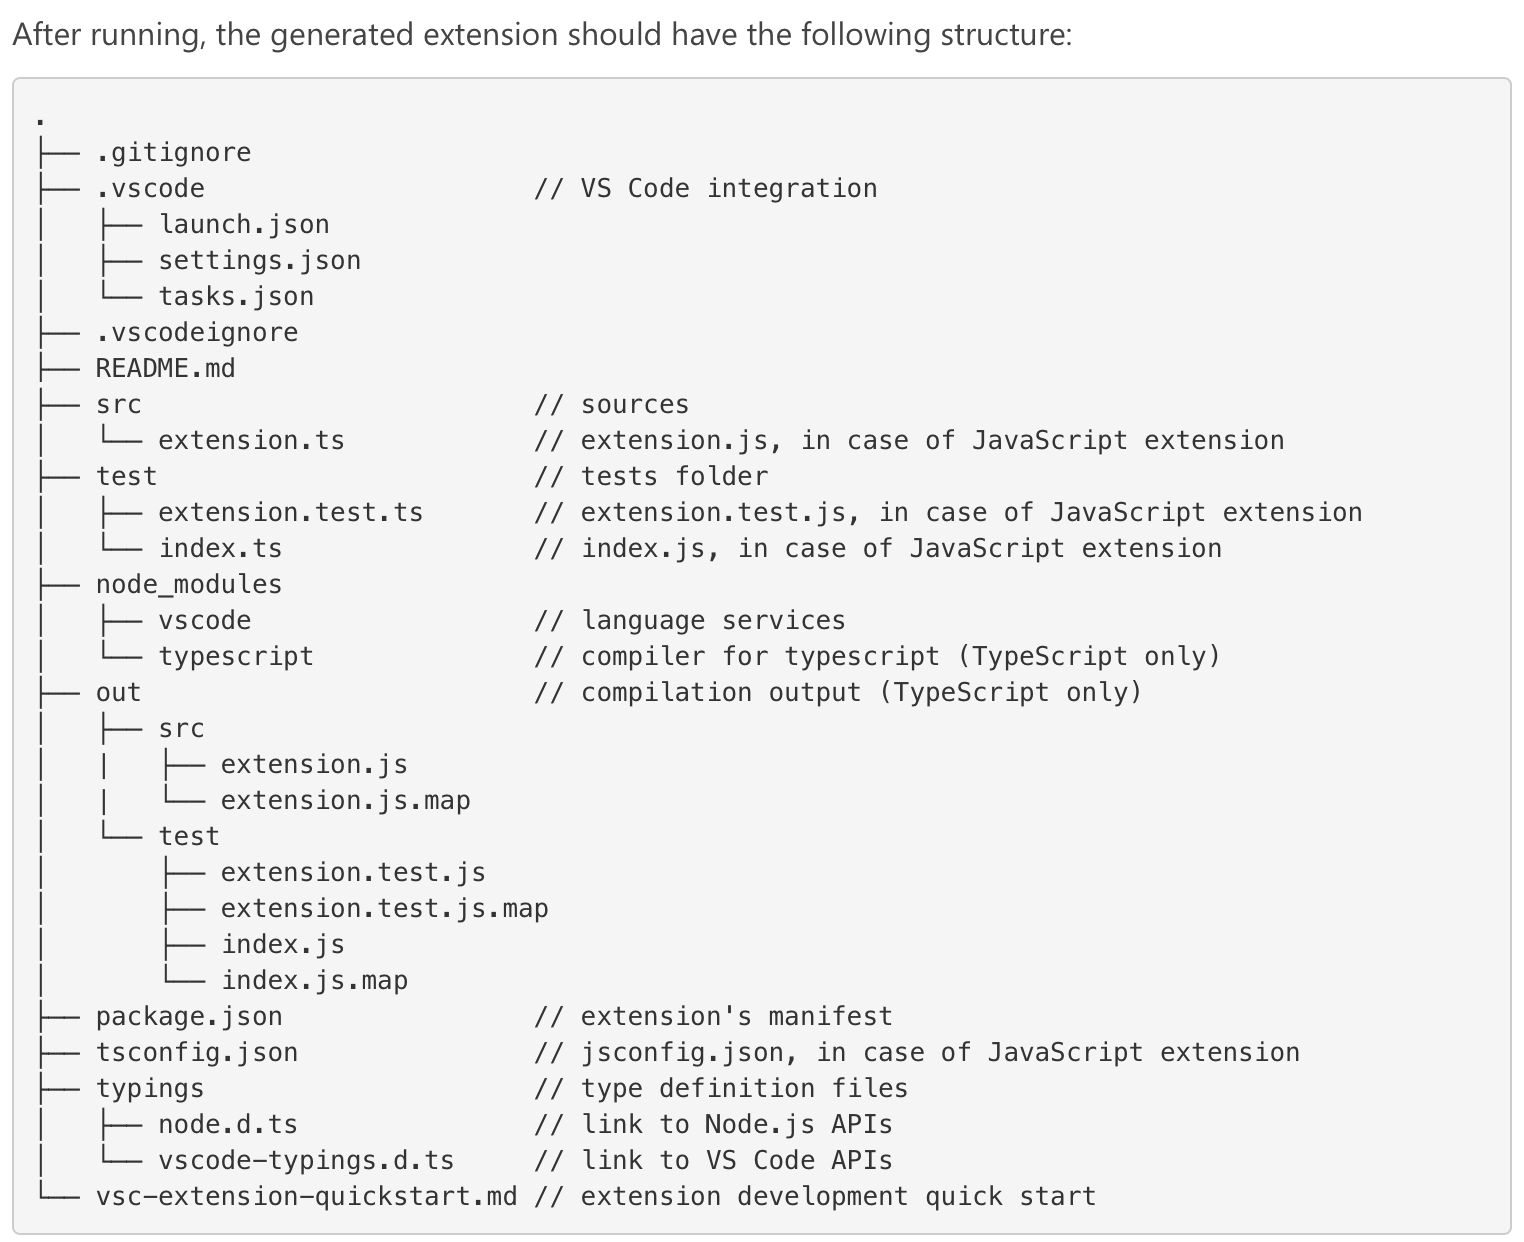
\includegraphics[scale=0.5]{fileStructure.png}
\caption{Basic file structure for a VS Code extension}
\end{figure}

\subsubsection{Operations}
Postal will have two main modes of operation.
The first being the active parsing, and the second being the file map mode.
The parsing mode is an unattended operation. As the user saves their files, the parser will parse and analyze the text checking for errors or malpractices as defined by W3C.
The second mode of operation an interactive mode. The user will utilize the visual file map to navigate to files, to visualize the file structure, and to locate the errors that the extension specifies within the code. 
All of these functions are partly data processing and support functions. 
The main goal of the extension is to process data using IFT design patterns.

\subsection{Product Functions}
From a functional perspective, Postal will largely do two things: Provide the user with a visual perspective of their project folder and parse HTML, CSS and JavaScript files for bad coding practices and information to feed into the visual interface. 
The visual interface component will be a separate window referred to as the `File Map'.
This window will scan the directory of the currently open project and create a visual representation of the files in the folder.
The representation will also feature indicators of errors that the parser detects in files and visually display any links between files.
The parser will read the HTML, CSS and JavaScript files in the user's project folder and look for specific violations of rules the defined in the system.
These rules will be based on the W3C best practices guidelines.
Additionally, the parser will ignore any lines of code that marked in an exception list, allowing the user to break rules in the case that they have to.
Along with our product completing the aforementioned requirements, it also needs to be implemented using the IFT Design Patterns also mentioned previously in this document.
The extension will be able to parse and interpret code projects with up to one hundred thousand lines of code quickly without noticeable lag. 
More specifically the extension will be able to handle files of this size with less than one second of lag.
The entire extension should run seamlessly with the user taking little to no notice that our processes are running. 
The user should experience little to no lag while our extension is running depending on the power of their personal machine.
This project will assume that an average user is using a computer with at least two gigabytes of ram. 
The project inherently won't have any safety requirements. 

\subsection{User Characteristics}
Users of Postal will be web developers and computer science students with some level of prior development experience, though prior knowledge will not be required. 
The users will be familiar with the concepts surrounding programming languages and markup languages, such as HTML, CSS and JavaScript. 
Users will be familiar with file systems, such that the visualization within Postal will enhance understanding of project structure. 
Users should have a basic understanding of debugging techniques that will be aided by the error recognition and highlighting within Postal.

\subsection{Constraints}
The Postal extension for VSC will be constrained chiefly by software and programming language level barriers.
As this extension will be primarily written in JavaScript (ECMAScript2016 standard, specifically), it will be bound by any functional or design limitations that exist within that programming language. 
Additionally, all Postal functionality must be possible within the VSC environment. 
VSC does not detail any notable performance constraints in its documentation that would conflict with the goals of Postal at this time. 
VSC does specify that extensions are not allowed access to the underlying UI DOM.
Finally, the file visualization and linking features of postal will be reliant on read, write and execute permissions within the scope of project loaded into VSC at that time.
If any user's operating system restricts Postal access to any of those file system features, that operating system will also be a constraint to proper function.

\subsection{Assumptions and Dependencies}
The successful development of Postal assumes that Microsoft will not update Visual Studio Code in such a manner that breaks the function of the Postal extension. 
It is also assumed that VSC will continue to support the operating systems used in development, testing, and utilization of Postal.

\subsection{Apportionment of Requirements}
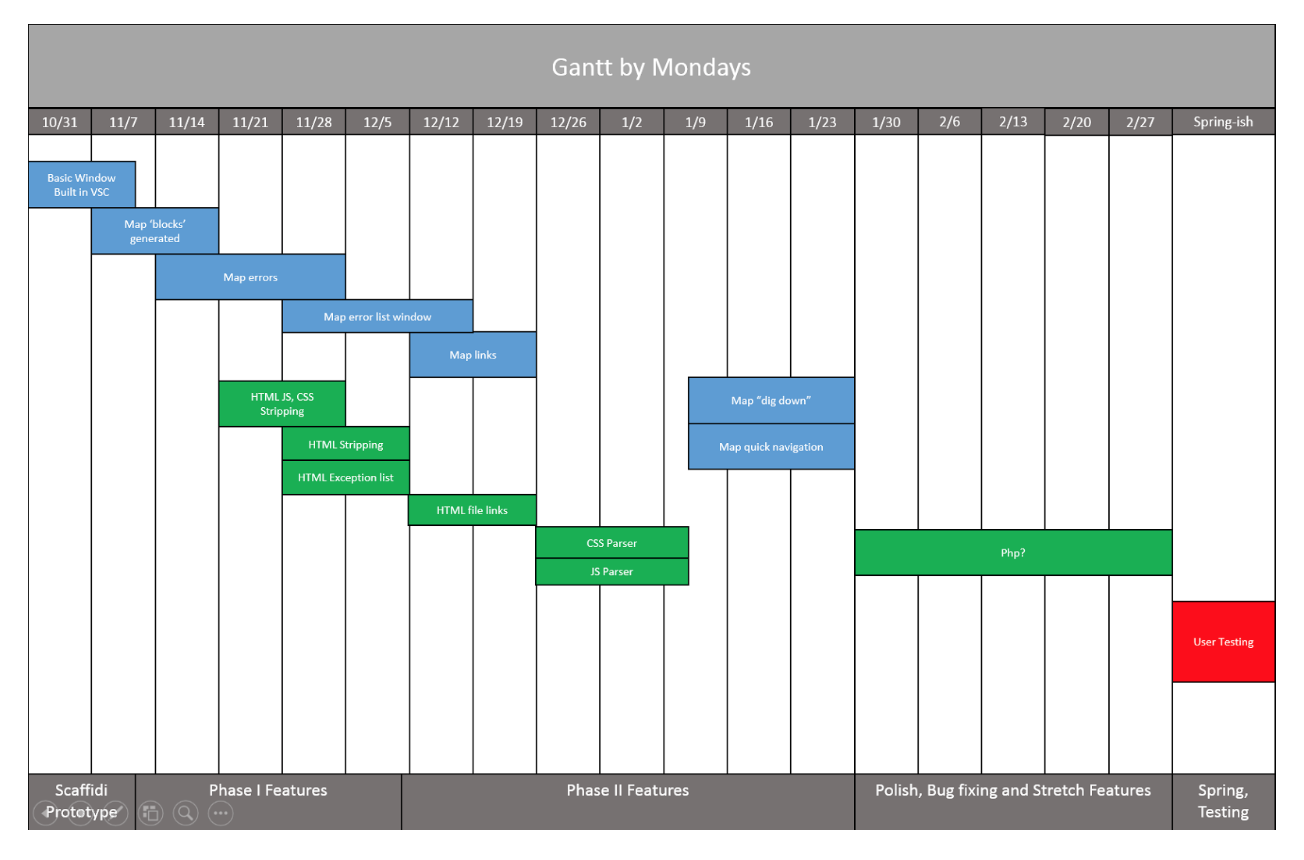
\includegraphics[scale=0.7]{gantt.png}

\section{Specific Requirements}

\subsection{External Interfaces}
The primary interface of the extension will be a window within the Visual Studio Code environment.
This window will contain two main elements (the File Map and the Error List) as well as a toolbar for options.
\\
The File Map is a visualization of the user's project.
When a project is opened within VSC, the extension will automatically populate the map by scanning the directory of the opened solution. 
This map will display each file found in the project directory in an organized fashion.
The map will also feature options to display a visual indicator of links and calls between files in the directory (for example, if an HTML page has an image embedded in it, the link option would indicate a link between the HTML and image files) as well as an option to display an indicator of the location of errors within the GUI.
\\
The user will also be able to interact with the File Map by ``digging down'' into a file.
This process will allow a user to click on a visualized file and have the map display more details about that file. 
For example, if an HTML file is clicked on within the map, the UI will update and visualize details of the file like divs and links as their own objects.
If the above mentioned error option is enabled, the object containing the error would indicate that.
\\
The Error list is a list which displays all errors that the parser detected during its last run.
The user will be able to click on a particular error in this list which will then trigger the extension to navigate the user to that particular error in the code. Additionally, if the user hovers over a particular error, the corresponding location in the file map will be highlighted.

\subsection{Functions}

\subsubsection{Parser Related Functionality}
\begin{itemize}
	\item Functionality capable of parsing JavaScript, HTML and CSS documents. 
	As parsing occurs, particular instances of code that break rules defined in the system will be flagged. 
	Flagged lines will be visualized in the File Map.
	\item The system must have a method for storing rules that will be used by the parser to determine if a line of code should be marked as an error.
	Many of these rules will be based on W3C best practices for the particular parser.
	\item The system must have an editable list of exceptions. 
	Exceptions are defined segments of code that may break a parsing rule, but because it was either intentional or necessary, should not throw an error.
	\item Current Parsing Rules for HTML:
		\begin{itemize}
			\item Flag JavaScript and CSS code that is not in the exception list.
			\item Make a note of each use of another file within the HTML file. This will be used to visualize links between files in the map.
		\end{itemize}
	\item Current Parsing Rules for CSS:
		\begin{itemize}
			\item Flag styles that can be optimized (ids vs. Classes).
			\item Flag redundant definitions.
			\item Do not flag code in the exception list.
		\end{itemize}
	\item Current Parsing Rules for JS:
		\begin{itemize}
			\item Flag Global variables that are not defined at the top of a file.
		\end{itemize}
\end{itemize}

\subsubsection{File Map Functionality}
\begin{itemize}
	\item Display in a visual, chart-like manner all files in the project directory.
    \item Display links and calls between files. This option can be turned off by the user.
    \item Display indicators of errors (broken rules) at the corresponding location within the map.
	 This option can be turned off by the user.
    \item The system must allow for the Dig Down functionality.
	 When an object in the map is clicked on, the map will update to display the object in more detail. Details will often be their own object.
	 Error indicators will be updated.
    \item Display an error list adjacent to the file map.
	 Errors will be organized by location.
    \begin{itemize}
    	\item If the user hovers over a particular error in the list, the corresponding location in the file map will be highlighted.
        \item If the user clicks on a particular error in the list, the extension will navigate the user to the location of the error in the code.
    \end{itemize}
\end{itemize}

\begin{figure}
\centering
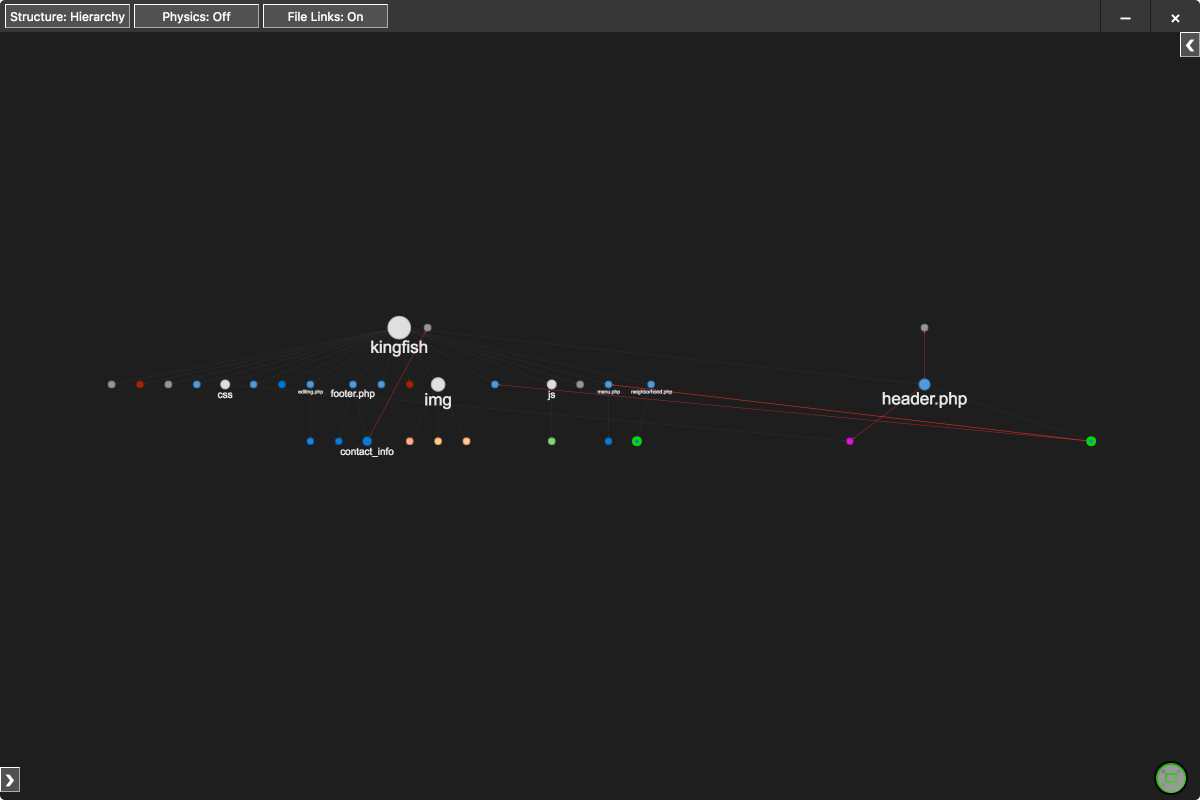
\includegraphics[scale=0.25]{filemap.png}
\caption{A mockup of what the file map could look like. 
In this example HTML pages are blue, CSS pages are navy, image files are purple and JavaScript files are green.
Red dots indicate that the parser found a broken rule in the file.}

\includegraphics[scale=0.25]{links.png}
\caption{A mockup of the link feature in the file map.
The Homepage.html file is `selected' and all links to other files are shown via arrows.
Note that files like Application2.js are greyed out as they do not have a link to the selected file.}

\pagebreak

\includegraphics[scale=0.25]{digdown.png}
\caption{An example of what a `dug into' Hompage.html file could look like.
In this example, the visual is expanded to the next level down of HTML tags.
These details may be expanded themselves.The error indicator from previous examples is also present and in this case states that the parse found an error in the Body section of the HTML document.}
\end{figure}

\subsection{Performance Requirements}
Our product will be able to support as many projects as each user has. 
Given a web site project consisting of less than thirty HTML files, five CSS files, and ten JavaScript files, our product should complete its analysis in less than a second. 
This example should be a pretty standard setup for most intermediate web developers.
\\
Our parser should complete each HTML file in less than 1/5th of a second and each CSS and JavaScript file in less than 1/10th of a second.

\subsubsection{Standards Compliance}
Other than the standards set forth by the VSC extension API, there are no overarching standards our product needs to comply with.
The plan is to test our product with people following the IRB protocols, and the testing will follow their safety requirements regarding the testers information.

\subsection{Software System Attributes}
The software that we will use is Visual Studio Code. We are making an extension for this base

\subsubsection{Reliability}
Postal should complete its analysis for 95\% of the projects it is given. It should also satisfy the performance requirements 95\% of the time.   

\subsubsection{Availability}
The extension will always be available as long as it is accessible from the VS Code Extension Marketplace. 
It will not need to pull any data from the internet for it to function, so it should always be available.

\subsubsection{Security}
The Postal extension will only save data that the user defines as setting of the application. 
The extension will know nothing of the user, and therefore will have nothing to be kept secure.

\subsubsection{Maintainability}
Postal will be implemented using Object Oriented Programming techniques which will aid in the maintainability of the software. 
This will mean if one section of the code is changed that is used in multiple places it will only need to be changed in once instead of each of those places.

\subsubsection{Portability}
The Postal extension will be written in JavaScript and will be able to be run on any computer that is able to run Visual Studio Code. 
The development will focus mainly on the Windows and Mac OSX operating systems, with minor testing in some variants of Linux.

\end{document}
